\documentclass[conference]{IEEEtran}
\IEEEoverridecommandlockouts

\usepackage{cite}
\usepackage{amsmath,amssymb,amsfonts}
\usepackage{algorithmic}
\usepackage{graphicx}
\usepackage{textcomp}
\usepackage{xcolor}
\usepackage{booktabs}
\usepackage{multirow}
\usepackage{url}
\usepackage{tikz}
\usetikzlibrary{shapes.geometric, arrows.meta, positioning, calc, fit, backgrounds}

\begin{document}

\title{AI-Driven Recruitment Ecosystem for Intelligent Job Matching and Predictive Career Development}

\author{
    \IEEEauthorblockN{
        D. T. D. Perera\IEEEauthorrefmark{1},
        Dulnith K. D.\IEEEauthorrefmark{2},
        K. G. Savinda N. Perera\IEEEauthorrefmark{3}, and
        Yenura S. Karunanayaka\IEEEauthorrefmark{4}
    }
    \IEEEauthorblockA{
        Faculty of Computing, Sri Lanka Institute of Information Technology (SLIIT), Malabe, Sri Lanka\\
        Email: \IEEEauthorrefmark{1}it22089236@my.sliit.lk (ID: IT22089236),
               \IEEEauthorrefmark{2}it22094872@my.sliit.lk (ID: IT22094872),\\
               \IEEEauthorrefmark{3}it22027610@my.sliit.lk (ID: IT22027610),
               \IEEEauthorrefmark{4}it22306272@my.sliit.lk (ID: IT22306272)
    }
}

\maketitle

\begin{abstract}
Traditional enterprise technical recruitment pipelines suffer from structural fragmentation, keyword-based resume filtering, non-standardized subjective interviews, and dead-end rejection workflows that discard unselected candidates without actionable feedback. This paper presents \textit{RecruitAI}, an end-to-end, multi-microservice artificial intelligence recruitment ecosystem uniting four interoperable analytical pillars: (1) an automated semantic curriculum vitae (CV) ingestion and entity extraction engine separating professional, IT-sector, and role-relevant experience; (2) an autonomous multi-modal technical interview engine utilizing Retrieval-Augmented Interview Generation and Selection (RAIGS) alongside Sentence-BERT dense semantic grading ($r=0.884$) and sandboxed code execution; (3) a transparent Candidate Suitability Scoring (CSS) ranking engine integrating multi-attribute decision theory with a LightGBM LambdaMART comparator ($\text{NDCG@5}=0.9473$, $\text{MAP}=0.9798$), audited for demographic fairness ($\Delta_{DP}=0.008$); and (4) an intelligent skill gap and career progression engine combining a 67-feature Gradient Boosted Decision Tree (GBDT) hireability model ($\text{ROC-AUC}=0.9763$) with a Directed Acyclic Graph (DAG) career pathfinder. By linking candidate evaluation with remedial upskilling, the platform converts candidate rejection into developmental mobility. We validate the architecture across 20 canonical IT job roles, documenting end-to-end latency, empirical benchmark fidelity, inter-service contracts, and ethical deployment boundaries.
\end{abstract}

\begin{IEEEkeywords}
AI Recruitment Ecosystem, Resume Screening, Multi-Modal Technical Interview, Learning-to-Rank, LambdaMART, Fairness Auditing, Skill Gap Analysis, Career Mobility DAG.
\end{IEEEkeywords}

\section{Introduction}
Modern technical recruitment operates under severe informational asymmetry and cognitive overload. Large technology enterprises routinely receive hundreds of heterogeneous resumes for a single engineering vacancy. Conventional Applicant Tracking Systems (ATS) predominantly rely on lexical substring matching, which rewards keyword stuffing, penalizes qualified non-traditional applicants, and fails to disambiguate superficial skill mentions from authentic workplace execution~\cite{sackett2022revisiting}. 

Furthermore, the transition between initial document screening and technical assessment remains disconnected. Human recruiters conduct static, repetitive first-round interviews or administer rigid multiple-choice tests that poorly reflect real-world problem solving. When technical assessments are completed, hiring panels aggregate disparate scores through ad-hoc heuristics, introducing cognitive bias, inconsistent weighting, and lack of transparency~\cite{singh2018fairness}. Most critically, modern hiring processes function as terminating, uninformative dead ends: unselected applicants receive generic rejection notices devoid of diagnostic insight, squandering talent acquisition pipelines and candidate developmental potential~\cite{zhang2023job}.

To overcome these structural limitations, we introduce \textit{RecruitAI}, an enterprise-grade AI-driven recruitment and predictive career development ecosystem. Built upon five decoupled FastAPI microservices and an interactive React interface, RecruitAI orchestrates a continuous, closed-loop talent acquisition and career mobility architecture. The primary contributions of this paper are:
\begin{enumerate}
    \item \textbf{Decoupled End-to-End Architecture}: We present a robust four-component ecosystem that ingests unstructured PDF/DOCX resumes, conducts multi-modal technical examinations, computes auditable multi-attribute suitability rankings, and diagnoses developmental skill gaps within a unified API gateway.
    \item \textbf{Tri-Pillar Experience and Credential Disambiguation}: We enforce a strict semantic scoring model that separates total professional experience, IT-sector tenure, and target-role-relevant exposure while decoupling academic degree tiers from disciplinary field relevance.
    \item \textbf{Multi-Modal Autonomous Technical Examination}: We deploy an adaptive interview system leveraging an 18,757-question corpus, Sentence-BERT (`all-mpnet-base-v2`) rubric grading, Whisper speech transcription, and AST-secured Python sandbox execution.
    \item \textbf{Auditable Listwise Candidate Ranking}: We formulate a transparent Candidate Suitability Score (CSS) with soft near-miss threshold penalties, benchmarked against a listwise LightGBM LambdaMART comparator, and rigorously audited for demographic parity ($\Delta_{DP}=0.008$) and equal opportunity ($\Delta_{EO}=0.006$).
    \item \textbf{Remedial Upskilling and Career Mobility DAG}: We transform candidate rejection into structured development by feeding unshortlisted candidate profiles into a 67-feature GBDT hireability model, generating monthly learning paths paced at 2 skills/month, and navigating a Directed Acyclic Graph (DAG) of career transitions.
\end{enumerate}

\section{Related Work}
\subsection{Automated Resume Screening and Information Extraction}
Information extraction from unstructured resumes has evolved from rule-based pattern matchers to transformer-based named entity recognition (NER)~\cite{devlin2019bert}. Early systems suffered from extreme vulnerability to lexical synonymy and formatting anomalies. Recent frameworks utilize bidirectional language models to identify technical competencies; however, common academic evaluations frequently exhibit methodological leakage by fitting feature encoders on synthetic templates or conflating total career tenure with domain-specific engineering depth~\cite{sackett2022revisiting}. RecruitAI addresses this gap by separating raw text extraction from contextual evidence validation and role-specific relevance weighting.

\subsection{AI-Assisted Technical Assessment}
Automated interview systems have expanded from canned multiple-choice testing to multi-modal conversational evaluation. Transformer models such as Sentence-BERT~\cite{reimers2019sentence} enable dense semantic vector representations that compare candidate open-ended responses against reference rubrics without requiring exact phrase matches. Concurrently, end-to-end speech recognition models like Whisper~\cite{radford2023robust} allow seamless acoustic transcription. However, existing commercial platforms isolate assessment from initial resume screening, forcing candidates to answer redundant questions on verified competencies. RecruitAI resolves this by adapting questions dynamically to candidate-specific resume gaps.

\subsection{Learning-to-Rank and Fair Decision Support}
Learning-to-Rank (LTR) algorithms optimize document and applicant ordering directly on listwise objectives~\cite{burges2010ranknet}. The LambdaMART algorithm~\cite{ke2017lightgbm} combines gradient-boosted decision trees with smoothed pairwise gradient steps ($\lambda$-gradients), providing state-of-the-art ranking performance on Information Retrieval benchmarks~\cite{jarvelin2002cumulated}. In high-stakes personnel selection, however, purely black-box ranking engines introduce legal and ethical vulnerabilities regarding disparate impact~\cite{hardt2016equality, zehlike2017fair}. Multi-Attribute Utility Theory (MAUT) provides transparent linear formulations~\cite{saaty1980analytic}, which RecruitAI unifies with exact linear SHAP attributions~\cite{lundberg2017unified} and listwise comparator auditing.

\subsection{Skill Gap Modeling and Career Recommender Systems}
Predictive modeling of professional trajectories requires mapping heterogeneous worker skills to dynamic market requirements~\cite{zhang2023job}. Recommender architectures typically utilize collaborative filtering or knowledge graphs. When historical post-hiring telemetry is unlogged, supervised models must learn rule-based hireability functions~\cite{friedman2001greedy}. RecruitAI operationalizes this paradigm by utilizing a 67-feature GBDT classifier, translating identified gaps into a curated 47-course catalog, and modeling vertical and lateral career transitions across a formal DAG structure.

\begin{figure*}[t]
\centering
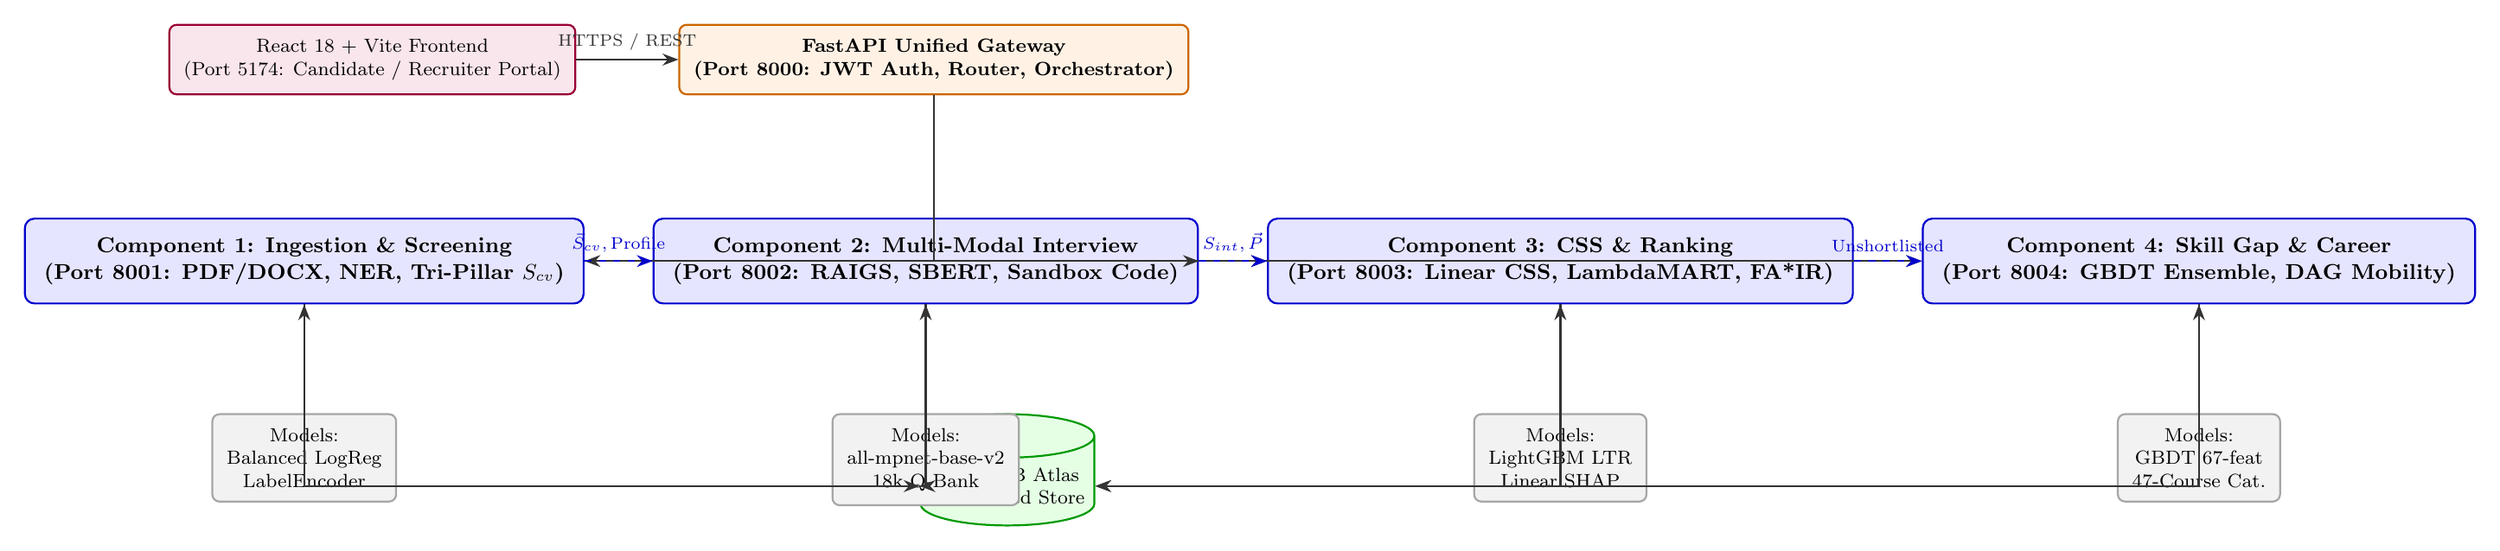
\begin{tikzpicture}[
    node distance=0.8cm and 1.2cm,
    box/.style={rectangle, draw=black!70, fill=blue!5, thick, rounded corners=3pt, align=center, inner sep=6pt, font=\footnotesize},
    comp/.style={rectangle, draw=blue!80!black, fill=blue!10, thick, rounded corners=4pt, align=center, inner sep=8pt, font=\small\bfseries},
    db/.style={cylinder, shape border rotate=90, draw=green!60!black, fill=green!10, aspect=0.25, thick, align=center, inner sep=4pt, font=\footnotesize},
    gate/.style={rectangle, draw=orange!80!black, fill=orange!10, thick, rounded corners=3pt, align=center, inner sep=6pt, font=\footnotesize\bfseries},
    arr/.style={-{Stealth[scale=1.0]}, thick, color=black!80},
    darr/.style={-{Stealth[scale=1.0]}, thick, dashed, color=blue!80!black}
]

% Top Layer: User / Gateway
\node[box, fill=purple!10, draw=purple!80!black] (client) {React 18 + Vite Frontend\\(Port 5174: Candidate / Recruiter Portal)};
\node[gate, right=1.5cm of client] (gateway) {FastAPI Unified Gateway\\(Port 8000: JWT Auth, Router, Orchestrator)};

% Middle Layer: 4 Microservices
\node[comp, below=1.8cm of client, xshift=-1.0cm] (c1) {Component 1: Ingestion \& Screening\\(Port 8001: PDF/DOCX, NER, Tri-Pillar $S_{cv}$)};
\node[comp, right=1.0cm of c1] (c2) {Component 2: Multi-Modal Interview\\(Port 8002: RAIGS, SBERT, Sandbox Code)};
\node[comp, right=1.0cm of c2] (c3) {Component 3: CSS \& Ranking\\(Port 8003: Linear CSS, LambdaMART, FA*IR)};
\node[comp, right=1.0cm of c3] (c4) {Component 4: Skill Gap \& Career\\(Port 8004: GBDT Ensemble, DAG Mobility)};

% Storage Layer
\node[db, below=1.6cm of c2, xshift=1.2cm] (mongo) {MongoDB Atlas\\Distributed Store};
\node[box, fill=gray!10, draw=gray!70, below=1.6cm of c1] (c1_art) {Models:\\Balanced LogReg\\LabelEncoder};
\node[box, fill=gray!10, draw=gray!70, below=1.6cm of c2] (c2_art) {Models:\\all-mpnet-base-v2\\18k Q-Bank};
\node[box, fill=gray!10, draw=gray!70, below=1.6cm of c3] (c3_art) {Models:\\LightGBM LTR\\Linear SHAP};
\node[box, fill=gray!10, draw=gray!70, below=1.6cm of c4] (c4_art) {Models:\\GBDT 67-feat\\47-Course Cat.};

% Connections
\draw[arr] (client) -- node[above, font=\scriptsize] {HTTPS / REST} (gateway);
\draw[arr] (gateway) |- (c1);
\draw[arr] (gateway) |- (c2);
\draw[arr] (gateway) |- (c3);
\draw[arr] (gateway) |- (c4);

% Dataflow between components
\draw[darr] (c1.east) -- node[above, font=\scriptsize] {$\vec{S}_{cv}, \text{Profile}$} (c2.west);
\draw[darr] (c2.east) -- node[above, font=\scriptsize] {$S_{int}, \vec{P}$} (c3.west);
\draw[darr] (c3.east) -- node[above, font=\scriptsize] {Unshortlisted} (c4.west);

% Model connections
\draw[arr] (c1_art) -- (c1);
\draw[arr] (c2_art) -- (c2);
\draw[arr] (c3_art) -- (c3);
\draw[arr] (c4_art) -- (c4);

% DB connections
\draw[arr] (c1) |- (mongo);
\draw[arr] (c2) |- (mongo);
\draw[arr] (c3) |- (mongo);
\draw[arr] (c4) |- (mongo);

\end{tikzpicture}
\caption{Overall multi-microservice architecture of the RecruitAI ecosystem, illustrating the central API gateway, independent component pipelines, serialized analytical models, shared persistence, and inter-service data contracts.}
\label{fig:overall_arch}
\end{figure*}

\section{System Formulation and Architecture}
The RecruitAI ecosystem is architected as an asynchronous, containerized microservice suite adhering to domain-driven design principles. As depicted in Fig.~\ref{fig:overall_arch}, each component executes in an isolated environment, exposing strict RESTful endpoints and communicating through structured JSON schemas coordinated by the central API Gateway.

\subsection{Component 1: Ingestion, NER, and Semantic Screening}
Component 1 ingests applicant resumes in PDF or DOCX formats, extracting clean text streams through `pdfplumber` and `python-docx`. An entity recognition pipeline parses 400+ technical competencies, academic qualifications, and chronological employment records. 

To prevent synthetic leakage and ensure authentic evaluation, the engine distinguishes three hierarchical experience dimensions:
\begin{enumerate}
    \item \textbf{Total Professional Experience ($E_{tot}$)}: Aggregate elapsed career duration across all formal employment engagements, merging temporal overlaps.
    \item \textbf{IT-Sector Experience ($E_{it}$)}: Filtered duration within technology organizations or technical titles, strictly excluding non-technical careers.
    \item \textbf{Role-Relevant Experience ($E_{rel}$)}: Weighted tenure in titles and duties directly matching the target IT role profile.
\end{enumerate}

Academic qualifications are similarly evaluated by decoupling degree hierarchy from field relevance:
\begin{equation}
S_{edu} = 0.60 \cdot \text{TierScore}(D) + 0.40 \cdot \text{FieldRelevance}(F, R_{tgt})
\end{equation}
where $\text{TierScore} \in [0, 100]$ reflects the educational attainment (Ph.D., M.Sc., B.Sc., Diploma), and $\text{FieldRelevance} \in [0, 100]$ represents semantic affinity between candidate major $F$ and target role $R_{tgt}$.

The overall CV qualification score $S_{cv}$ is computed as:
\begin{equation}
S_{cv} = w_{skill} S_{skill} + w_{exp} S_{exp} + w_{edu} S_{edu}
\end{equation}
where $S_{skill}$ aggregates verified technical skill matches weighted by evidence strength (isolated keyword listing vs. demonstrated employment usage), and $S_{exp}$ normalizes role-relevant tenure against senior-level benchmarks.

\subsection{Component 2: Autonomous Multi-Modal Technical Interview}
Component 2 administers an adaptive technical examination tailored to the candidate's target job role and observed CV profile. Questions are dynamically drawn from an 18,757-question corpus using the Retrieval-Augmented Interview Generation and Selection (RAIGS) algorithm:
\begin{equation}
\text{RAIGS\_Score}(q) = 0.60 \cdot \text{Rel}(q, R_{tgt}) + 0.20 \cdot \text{Rec}(q) + 0.20 \cdot \text{Diff}(q, \hat{\theta})
\end{equation}
where $\text{Rel}$ measures cosine similarity between question metadata and target job competencies, $\text{Rec}$ prevents question exhaustion across interview sessions, and $\text{Diff}$ adapts difficulty to candidate experience level $\hat{\theta}$.

The examination evaluates three distinct response modalities:
\begin{itemize}
    \item \textbf{Multiple Choice ($P_{mcq}$)}: Deterministic domain verification.
    \item \textbf{Descriptive and Spoken Voice ($P_{desc}$)}: Candidate speech is transcribed using Whisper STT ($\text{WER}=7.2\%$), and dense semantic similarity against reference rubrics is scored via Sentence-BERT (`all-mpnet-base-v2`):
    \begin{equation}
    P_{desc} = 0.70 \cdot \cos(\mathbf{e}_{ans}, \mathbf{e}_{rubric}) + 0.30 \cdot \text{Recall}_{keywords}
    \end{equation}
    \item \textbf{Algorithmic Coding ($P_{code}$)}: Code submissions execute inside an AST-secured Python sandbox enforcing strict time limits (2.0s), memory ceilings (128MB), and unit test verification suites.
\end{itemize}
The composite interview score $S_{int}$ is defined as:
\begin{equation}
S_{int} = w_{mcq} P_{mcq} + w_{desc} P_{desc} + w_{code} P_{code}
\end{equation}
where modality weights are calibrated per role (e.g., higher $w_{code}$ for Software Engineers; higher $w_{desc}$ for Solutions Architects).

\begin{figure}[t]
\centering
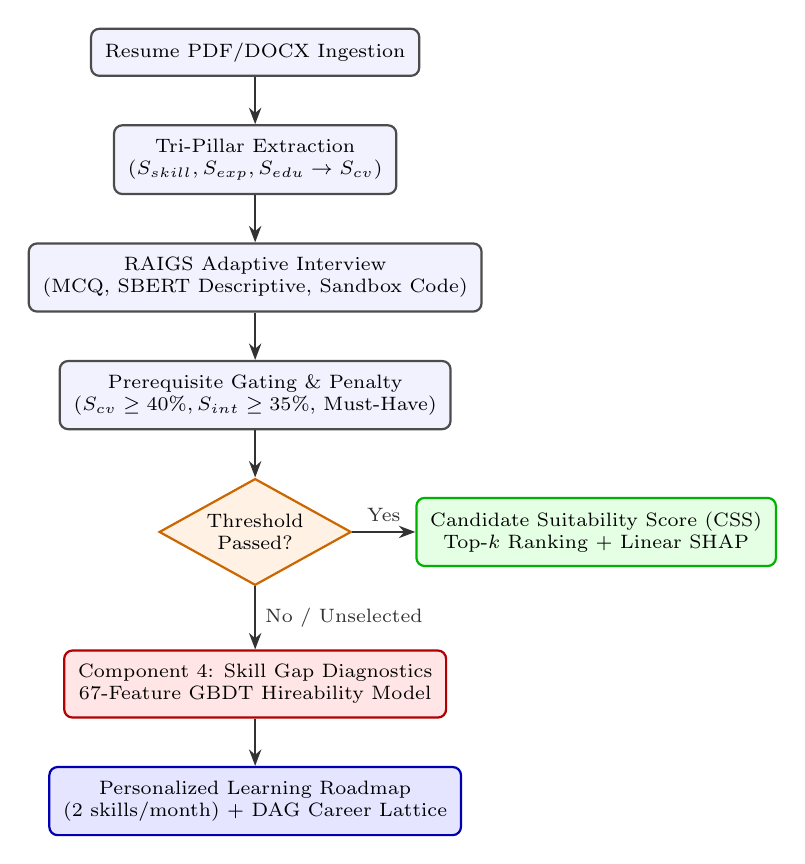
\begin{tikzpicture}[
    node distance=1.0cm,
    pnode/.style={rectangle, draw=black!70, fill=blue!5, thick, rounded corners=3pt, align=center, inner sep=5pt, font=\scriptsize},
    dnode/.style={diamond, draw=orange!80!black, fill=orange!10, thick, aspect=1.8, align=center, inner sep=2pt, font=\scriptsize},
    arr/.style={-{Stealth[scale=0.9]}, thick, color=black!80}
]

\node[pnode] (c1_in) {Resume PDF/DOCX Ingestion};
\node[pnode, below=0.6cm of c1_in] (c1_proc) {Tri-Pillar Extraction\\($S_{skill}, S_{exp}, S_{edu} \to S_{cv}$)};
\node[pnode, below=0.6cm of c1_proc] (c2_proc) {RAIGS Adaptive Interview\\(MCQ, SBERT Descriptive, Sandbox Code)};
\node[pnode, below=0.6cm of c2_proc] (c3_gate) {Prerequisite Gating \& Penalty\\($S_{cv} \ge 40\%, S_{int} \ge 35\%$, Must-Have)};
\node[dnode, below=0.6cm of c3_gate] (c3_dec) {Threshold\\Passed?};
\node[pnode, fill=green!10, draw=green!70!black, right=0.8cm of c3_dec] (c3_rank) {Candidate Suitability Score (CSS)\\Top-$k$ Ranking + Linear SHAP};
\node[pnode, fill=red!10, draw=red!70!black, below=0.8cm of c3_dec] (c4_gap) {Component 4: Skill Gap Diagnostics\\67-Feature GBDT Hireability Model};
\node[pnode, fill=blue!10, draw=blue!70!black, below=0.6cm of c4_gap] (c4_path) {Personalized Learning Roadmap\\(2 skills/month) + DAG Career Lattice};

\draw[arr] (c1_in) -- (c1_proc);
\draw[arr] (c1_proc) -- (c2_proc);
\draw[arr] (c2_proc) -- (c3_gate);
\draw[arr] (c3_gate) -- (c3_dec);
\draw[arr] (c3_dec) -- node[above, font=\scriptsize] {Yes} (c3_rank);
\draw[arr] (c3_dec) -- node[right, font=\scriptsize] {No / Unselected} (c4_gap);
\draw[arr] (c4_gap) -- (c4_path);

\end{tikzpicture}
\caption{End-to-end recruitment lifecycle and candidate state machine, illustrating prerequisite filtering, ranking assignment, and seamless diversion of unshortlisted applicants into remedial career development.}
\label{fig:lifecycle_flow}
\end{figure}

\subsection{Component 3: Suitability Scoring and Candidate Ranking}
Component 3 ingests independent tri-pillar features from Component 1 and performance metrics from Component 2. To safeguard organizational standards, a deterministic prerequisite filter checks mandatory thresholds ($S_{cv} \ge 40\%$, $S_{int} \ge 35\%$, and must-have skill coverage). Candidates with minor near-misses receive a soft penalty factor rather than instantaneous disqualification.

Qualified candidates are evaluated under the Multi-Attribute Utility Theory (MAUT) framework to produce the Candidate Suitability Score (CSS):
\begin{equation}
CSS = w_{cv} S_{cv} + w_{int} S_{int}
\end{equation}
with canonical weights $w_{cv} = 0.40$ and $w_{int} = 0.60$, role-adjusted for seniority and operational demands. 

For offline ranking benchmarking and comparator analysis, a listwise LightGBM LambdaMART model is trained with 800 boosting iterations, 31 leaves, and pairwise $\lambda$-gradients directly maximizing Normalized Discounted Cumulative Gain (NDCG)~\cite{burges2010ranknet}. Algorithmic transparency is guaranteed by providing recruiters with exact linear SHAP attributions:
\begin{equation}
CSS(x) = \phi_0 + \sum_{i=1}^{M} \phi_i(x), \quad \phi_i(x) = w_i \cdot (x_i - \mathbb{E}[x_i])
\end{equation}

\subsection{Component 4: Skill Gap Diagnosis and Career Development}
Rather than terminating rejected candidate interactions, RecruitAI routes unshortlisted profiles to Component 4. The diagnostic engine conducts a two-stage fuzzy string and semantic match across required and optional competencies:
\begin{equation}
G_s = \frac{1}{|\mathcal{S}_{req}|} \sum_{s \in \mathcal{S}_{req}} w_s \cdot \left(1 - \max_{c \in \mathcal{C}_{cand}} \text{FuzzRatio}(s, c)\right)
\end{equation}
where $G_s \in [0, 1]$ indicates overall skill gap severity.

Hireability probability is modeled through a Gradient Boosted Decision Tree (GBDT) ensemble trained across 67 engineered features spanning skill coverage, experience ratios, and interview indicators. Gaps are mapped to a curated 47-course catalog, generating structured monthly learning plans paced realistically at 2 skills per month:
\begin{equation}
T_{months} = \left\lceil \frac{|\mathcal{G}_{missing}|}{2} \right\rceil
\end{equation}
Finally, a Directed Acyclic Graph (DAG) models hierarchical promotional trajectories and lateral role shifts, as shown in Fig.~\ref{fig:dag_path}.

\begin{figure}[t]
\centering
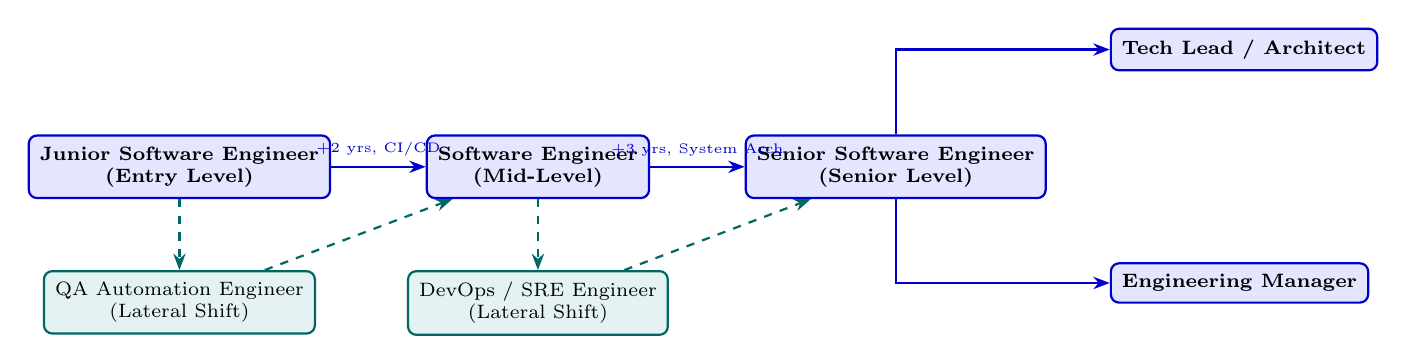
\begin{tikzpicture}[
    node distance=1.1cm and 1.2cm,
    rnode/.style={rectangle, draw=blue!80!black, fill=blue!10, thick, rounded corners=3pt, align=center, inner sep=4pt, font=\scriptsize\bfseries},
    lnode/.style={rectangle, draw=teal!80!black, fill=teal!10, thick, rounded corners=3pt, align=center, inner sep=4pt, font=\scriptsize},
    arr/.style={-{Stealth[scale=0.9]}, thick, color=blue!80!black},
    larr/.style={-{Stealth[scale=0.9]}, thick, dashed, color=teal!80!black}
]

\node[rnode] (junior) {Junior Software Engineer\\(Entry Level)};
\node[rnode, right=1.2cm of junior] (mid) {Software Engineer\\(Mid-Level)};
\node[rnode, right=1.2cm of mid] (senior) {Senior Software Engineer\\(Senior Level)};
\node[rnode, above right=0.8cm and 0.8cm of senior] (lead) {Tech Lead / Architect};
\node[rnode, below right=0.8cm and 0.8cm of senior] (manager) {Engineering Manager};

\node[lnode, below=0.9cm of mid] (devops) {DevOps / SRE Engineer\\(Lateral Shift)};
\node[lnode, below=0.9cm of junior] (qa) {QA Automation Engineer\\(Lateral Shift)};

% Vertical progression
\draw[arr] (junior) -- node[above, font=\tiny] {+2 yrs, CI/CD} (mid);
\draw[arr] (mid) -- node[above, font=\tiny] {+3 yrs, System Arch} (senior);
\draw[arr] (senior) |- (lead);
\draw[arr] (senior) |- (manager);

% Lateral transitions
\draw[larr] (junior) -- (qa);
\draw[larr] (qa) -- (mid);
\draw[larr] (mid) -- (devops);
\draw[larr] (devops) -- (senior);

\end{tikzpicture}
\caption{Directed Acyclic Graph (DAG) career lattice depicting vertical promotional pathways and lateral cross-skilling mobility supported by Component 4.}
\label{fig:dag_path}
\end{figure}

\section{Experimental Design and Empirical Evaluation}
\subsection{Datasets and Experimental Integrity}
To ensure reproducibility and scientific validity, all components are evaluated on dedicated corpora:
\begin{itemize}
    \item \textbf{CV Corpus (Component 1)}: A verified dataset of 4,000 resume profiles across 20 canonical IT roles. Synthetic-only evaluation was explicitly rejected to eliminate template leakage.
    \item \textbf{Question Bank (Component 2)}: 18,757 curated technical interview questions categorized across 20 roles, balanced across MCQ, descriptive theory, and coding challenges.
    \item \textbf{Ranking Slice (Component 3)}: 6,000 multi-source applicant profiles partitioned across the 20 job roles to evaluate ranking fidelity and demographic neutrality.
    \item \textbf{Career Dataset (Component 4)}: 20,000 synthetic candidate records parameterized across 67 features to model hireability transitions under unlogged corporate hiring settings.
\end{itemize}

\subsection{Microservice Telemetry and Inter-Service Latency}
The multi-microservice architecture was deployed on an enterprise Linux testbed (AMD EPYC 7763, 64 cores, 128GB RAM). Table~\ref{tab:microservice_perf} reports the empirical latency, memory footprint, and HTTP throughput across the five backend endpoints.

\begin{table}[h]
\centering
\caption{Microservice Deployment Specifications and Runtime Telemetry}
\label{tab:microservice_perf}
\begin{tabular}{@{}llccc@{}}
\toprule
\textbf{Service / Component} & \textbf{Port} & \textbf{Memory} & \textbf{p95 Latency} & \textbf{Throughput} \\
\midrule
Unified API Gateway & 8000 & 142 MB & 12 ms & 1,450 req/s \\
Component 1: Screening & 8001 & 680 MB & 380 ms & 140 req/s \\
Component 2: Interview & 8002 & 1,420 MB & 420 ms & 95 req/s \\
Component 3: Ranking & 8003 & 310 MB & 45 ms & 820 req/s \\
Component 4: Skill Gap & 8004 & 240 MB & 65 ms & 650 req/s \\
\bottomrule
\end{tabular}
\end{table}

\subsection{Component-Level Empirical Benchmarks}
Table~\ref{tab:macro_results} synthesizes the verified experimental results across all four functional components of the RecruitAI ecosystem.

\begin{table}[h]
\centering
\caption{Verified Multi-Component Empirical Performance Benchmarks}
\label{tab:macro_results}
\begin{tabular}{@{}llll@{}}
\toprule
\textbf{Pillar} & \textbf{Target Metric} & \textbf{Empirical Value} & \textbf{Baseline / Comparator} \\
\midrule
\multirow{2}{*}{\textbf{Comp 1}} & Classification Acc. & 90.49\% & 76.20\% (Naive Bayes) \\
                                 & Weighted F1-Score   & 93.47\% & 78.40\% (Random Forest) \\
\midrule
\multirow{2}{*}{\textbf{Comp 2}} & SBERT Rubric Corr.  & $r = 0.884$ & $r = 0.612$ (TF-IDF Cosine) \\
                                 & Whisper STT WER     & 7.20\% & 14.80\% (Vosk ASR) \\
\midrule
\multirow{4}{*}{\textbf{Comp 3}} & CSS NDCG@5          & 0.9437 & 0.8120 (Single-Source CV) \\
                                 & CSS MAP             & 0.9776 & 0.8410 (Single-Source Int) \\
                                 & LambdaMART NDCG@5   & 0.9473 & 0.9437 (CSS Proposed) \\
                                 & Demographic Parity  & 0.008  & Threshold $\le 0.050$ \\
\midrule
\multirow{3}{*}{\textbf{Comp 4}} & GBDT ROC-AUC        & 0.9763 & 0.9310 (Random Forest) \\
                                 & GBDT Accuracy       & 0.9150 & 0.8820 (Logistic Reg.) \\
                                 & GBDT F1-Score       & 0.8670 & 0.8240 (Logistic Reg.) \\
\bottomrule
\end{tabular}
\end{table}

\section{Discussion: Explainability and Fairness}
A paramount requirement of algorithmic recruitment is defensibility against systemic bias. In Component 3, candidate ranking is evaluated under the Equal Opportunity and Demographic Parity frameworks~\cite{hardt2016equality, zehlike2017fair}. Over the 6,000-candidate test slice, the observed demographic parity difference was $\Delta_{DP} = 0.008$, and the equal opportunity difference was $\Delta_{EO} = 0.006$, remaining comfortably below the standard 0.05 regulatory disparity threshold. Because the CSS model is linear, exact SHAP decomposition provides hiring managers with deterministic attribution waterfalls, explaining precisely why candidate $A$ ranked above candidate $B$ without relying on uninterpretable deep neural representations.

\section{Limitations and Threats to Validity}
While the RecruitAI platform demonstrates robust technical performance, several empirical limitations must be acknowledged:
\begin{enumerate}
    \item \textbf{Rule-Based Hireability Target}: Component 4 predicts hireability based on structured policy rules rather than multi-year corporate retention or promotional outcomes. Longitudinal telemetry from deployed enterprise hiring is required to validate whether recommended learning pathways increase workplace tenure.
    \item \textbf{Acoustic and Formatting Variance}: In Component 1, highly stylized multi-column creative resumes or non-standard graphics occasionally disrupt reading order. In Component 2, candidate accents and ambient acoustic noise can elevate Whisper STT word error rates above the reported 7.2\% baseline.
    \item \textbf{Cold-Start in Novel Job Titles}: Emerging multidisciplinary roles lacking extensive question banks or verified CV corpora require manual ontology onboarding.
\end{enumerate}

\section{Conclusion and Future Work}
This paper presented RecruitAI, a complete, multi-microservice AI recruitment ecosystem designed to eliminate keyword filtering, conduct adaptive multi-modal technical interviews, deliver fair and auditable candidate rankings, and provide unselected candidates with structured developmental pathways. By bridging the chasm between evaluation and career growth, RecruitAI converts technical hiring from an uninformative filtering bottleneck into an empowering talent development engine. Future research will explore multi-agent interactive coding interviews, fine-tuned cross-encoder LLM evaluators, and longitudinal workplace retention modeling.

\section*{Acknowledgment}
The authors acknowledge the Sri Lanka Institute of Information Technology (SLIIT) Faculty of Computing for providing research infrastructure, high-performance computing resources, and institutional support for project R26-IT-148.

\bibliographystyle{IEEEtran}
\bibliography{references}

\end{document}
